%%%%%%%%%%%%%%%%%%%%%%%%%%%%%%%%%%%%%%%%%%%%%%%%%%%%%%%%%%%%
% CAUTION:
% Need to compile under XeTex or XeLaTeX
%%%%%%%%%%%%%%%%%%%%%%%%%%%%%%%%%%%%%%%%%%%%%%%%%%%%%%%%%%%%

\documentclass{beamer}

%
% Common preamble for all three parts.
%

\usepackage[english]{babel}
\usepackage{amsmath}
\usepackage{color}
\usepackage{minted}
\usepackage{hyperref}
\usepackage{multicol}
\usepackage{tabularx}
\usepackage{tikz}

% only inline todonotes work
\usepackage{xkeyval}
\usepackage[textsize=small]{todonotes}
\presetkeys{todonotes}{inline}{}

\usetikzlibrary{shapes,arrows,positioning,shadows}

% no nav buttons
\usenavigationsymbolstemplate{}

\newcommand{\bftt}[1]{\textbf{\texttt{#1}}}
\newcommand{\comment}[1]{{\color[HTML]{008080}\textit{\textbf{\texttt{#1}}}}}
\newcommand{\cmd}[1]{{\color[HTML]{008000}\bftt{#1}}}
\newcommand{\bs}{\char`\\}
\newcommand{\cmdbs}[1]{\cmd{\bs#1}}
\newcommand{\lcb}{\char '173}
\newcommand{\rcb}{\char '175}
\newcommand{\cmdbegin}[1]{\cmdbs{begin\lcb}\bftt{#1}\cmd{\rcb}}
\newcommand{\cmdend}[1]{\cmdbs{end\lcb}\bftt{#1}\cmd{\rcb}}

\newcommand{\wllogo}{\textbf{Overleaf}}

% this is where the example source files are loaded from
% do not include a trailing slash
\newcommand{\fileuri}{https://raw.github.com/jdleesmiller/latex-course/master/en}

\newcommand{\wlserver}{https://www.overleaf.com}
\newcommand{\wlnewdoc}[1]{\wlserver/docs?snip\_uri=\fileuri/#1\&splash=none}

\def\tikzname{Ti\emph{k}Z}

% from http://tex.stackexchange.com/questions/5226/keyboard-font-for-latex
\newcommand*\keystroke[1]{%
  \tikz[baseline=(key.base)]
    \node[%
      draw,
      fill=white,
      drop shadow={shadow xshift=0.25ex,shadow yshift=-0.25ex,fill=black,opacity=0.75},
      rectangle,
      rounded corners=2pt,
      inner sep=1pt,
      line width=0.5pt,
      font=\scriptsize\sffamily
    ](key) {#1\strut}
  ;
}
\newcommand{\keystrokebftt}[1]{\keystroke{\bftt{#1}}}

% stolen from minted.dtx
\newenvironment{exampletwoup}
  {\VerbatimEnvironment
   \begin{VerbatimOut}{example.out}}
  {\end{VerbatimOut}
   \setlength{\parindent}{0pt}
   \fbox{\begin{tabular}{l|l}
   \begin{minipage}{0.55\linewidth}
     \inputminted[fontsize=\small,resetmargins]{latex}{example.out}
   \end{minipage} &
   \begin{minipage}{0.35\linewidth}
     \input{example.out}
   \end{minipage}
   \end{tabular}}}

\newenvironment{exampletwouptiny}
  {\VerbatimEnvironment
   \begin{VerbatimOut}{example.out}}
  {\end{VerbatimOut}
   \setlength{\parindent}{0pt}
   \fbox{\begin{tabular}{l|l}
   \begin{minipage}{0.55\linewidth}
     \inputminted[fontsize=\scriptsize,resetmargins]{latex}{example.out}
   \end{minipage} &
   \begin{minipage}{0.35\linewidth}
     \setlength{\parskip}{6pt plus 1pt minus 1pt}%
     \raggedright\scriptsize\input{example.out}
   \end{minipage}
   \end{tabular}}}

\newenvironment{exampletwouptinynoframe}
  {\VerbatimEnvironment
   \begin{VerbatimOut}{example.out}}
  {\end{VerbatimOut}
   \setlength{\parindent}{0pt}
   \begin{tabular}{l|l}
   \begin{minipage}{0.55\linewidth}
     \inputminted[fontsize=\scriptsize,resetmargins]{latex}{example.out}
   \end{minipage} &
   \begin{minipage}{0.35\linewidth}
     \setlength{\parskip}{6pt plus 1pt minus 1pt}%
     \raggedright\scriptsize\input{example.out}
   \end{minipage}
   \end{tabular}}

\title{An Interactive Introduction to \LaTeX}
\author{Dr John D. Lees-Miller}
\titlegraphic{%

\includegraphics[height=36pt]{Overleaf-logo-300dpi}\\[1em]

\includegraphics[height=24pt]{UoB-logo}
\qquad

\includegraphics[height=24pt]{setsquared_supported}
}


\subtitle{第二节:多层文档...}

\begin{document}

%%%%%%%%%%%%%%%%%%%%%%%%%%%%%%%%%%%%%%%%%%%%%%%%%%%%%%%%%%%%%%%%%%%%%%%%%%%%%%%
%%%%%%%%%%%%%%%%%%%%%%%%%%%%%%%%%%%%%%%%%%%%%%%%%%%%%%%%%%%%%%%%%%%%%%%%%%%%%%%
%%%%%%%%%%%%%%%%%%%%%%%%%%%%%%%%%%%%%%%%%%%%%%%%%%%%%%%%%%%%%%%%%%%%%%%%%%%%%%%
\begin{frame}
\titlepage
\end{frame}

%%%%%%%%%%%%%%%%%%%%%%%%%%%%%%%%%%%%%%%%%%%%%%%%%%%%%%%%%%%%%%%%%%%%%%%%%%%%%%%
%%%%%%%%%%%%%%%%%%%%%%%%%%%%%%%%%%%%%%%%%%%%%%%%%%%%%%%%%%%%%%%%%%%%%%%%%%%%%%%
%%%%%%%%%%%%%%%%%%%%%%%%%%%%%%%%%%%%%%%%%%%%%%%%%%%%%%%%%%%%%%%%%%%%%%%%%%%%%%%
\section{分层文档}

%%%%%%%%%%%%%%%%%%%%%%%%%%%%%%%%%%%%%%%%%%%%%%%%%%%%%%%%%%%%%%%%%%%%%%%%%%%%%%%
%%%%%%%%%%%%%%%%%%%%%%%%%%%%%%%%%%%%%%%%%%%%%%%%%%%%%%%%%%%%%%%%%%%%%%%%%%%%%%%
%%%%%%%%%%%%%%%%%%%%%%%%%%%%%%%%%%%%%%%%%%%%%%%%%%%%%%%%%%%%%%%%%%%%%%%%%%%%%%%
\begin{frame}{大纲}
\begin{multicols}{2}
\tableofcontents[currentsection]
\end{multicols}
\end{frame}

%%%%%%%%%%%%%%%%%%%%%%%%%%%%%%%%%%%%%%%%%%%%%%%%%%%%%%%%%%%%%%%%%%%%%%%%%%%%%%%
%%%%%%%%%%%%%%%%%%%%%%%%%%%%%%%%%%%%%%%%%%%%%%%%%%%%%%%%%%%%%%%%%%%%%%%%%%%%%%%
%%%%%%%%%%%%%%%%%%%%%%%%%%%%%%%%%%%%%%%%%%%%%%%%%%%%%%%%%%%%%%%%%%%%%%%%%%%%%%%
\begin{frame}{\insertsection}
\begin{itemize}
\item 在第一节,我们学习了一些命令和情境。它们能将文本和公式转换成各种格式。
\item 现在我们学习控制文档结构。这会用到另一些命令和情境。
\item 你可以在Overleaf中试试这些新命令:
\end{itemize}
\vskip 2em
\begin{center}
\fbox{\href{\wlnewdoc{basics.tex}}{%
点此打开\wllogo{}示例文档}}
\\[1ex]\scriptsize{}
为保证编译体验,最好使用 \href{http://www.google.com/chrome}{Google Chrome} 或新版 \href{http://www.mozilla.org/en-US/firefox/new/}{FireFox}浏览器。
\end{center}
\vskip 2ex
\begin{itemize}
\item 开始吧!
\end{itemize}
\end{frame}

%%%%%%%%%%%%%%%%%%%%%%%%%%%%%%%%%%%%%%%%%%%%%%%%%%%%%%%%%%%%%%%%%%%%%%%%%%%%%%%
%%%%%%%%%%%%%%%%%%%%%%%%%%%%%%%%%%%%%%%%%%%%%%%%%%%%%%%%%%%%%%%%%%%%%%%%%%%%%%%
%%%%%%%%%%%%%%%%%%%%%%%%%%%%%%%%%%%%%%%%%%%%%%%%%%%%%%%%%%%%%%%%%%%%%%%%%%%%%%%
\subsection{标题页和摘要}
\begin{frame}[fragile]{\insertsubsection}
\begin{itemize}{\small
\item 在头文件中告诉 \LaTeX{} 标题 \cmdbs{title} 和作者 \cmdbs{author}。
\item 然后在正文中用\cmdbs{maketitle} 生成标题。
\item 把摘要放在\bftt{abstract}情境里。
}\end{itemize}
\begin{minipage}{0.55\linewidth}
\inputminted[fontsize=\scriptsize,frame=single,resetmargins]{latex}%
  {ex-p2-struc-title.tex}
\end{minipage}
\begin{minipage}{0.35\linewidth}

\includegraphics[width=\textwidth,clip,trim=2.2in 7in 2.2in 2in]{ex-p2-struc-title.pdf}
\end{minipage}
\end{frame}

%%%%%%%%%%%%%%%%%%%%%%%%%%%%%%%%%%%%%%%%%%%%%%%%%%%%%%%%%%%%%%%%%%%%%%%%%%%%%%%
%%%%%%%%%%%%%%%%%%%%%%%%%%%%%%%%%%%%%%%%%%%%%%%%%%%%%%%%%%%%%%%%%%%%%%%%%%%%%%%
%%%%%%%%%%%%%%%%%%%%%%%%%%%%%%%%%%%%%%%%%%%%%%%%%%%%%%%%%%%%%%%%%%%%%%%%%%%%%%%
\subsection{章节}
\begin{frame}{\insertsubsection}
\begin{itemize}{\small
\item 使用 \cmdbs{section} 和 \cmdbs{subsection}分层即可。
\item 你猜 \cmdbs{section*} 和 \cmdbs{subsection*} 有什么效果?
}\end{itemize}
\begin{minipage}{0.55\linewidth}
\inputminted[fontsize=\scriptsize,frame=single,resetmargins]{latex}%
  {ex-p2-struc-sections.tex}
\end{minipage}
\begin{minipage}{0.35\linewidth}
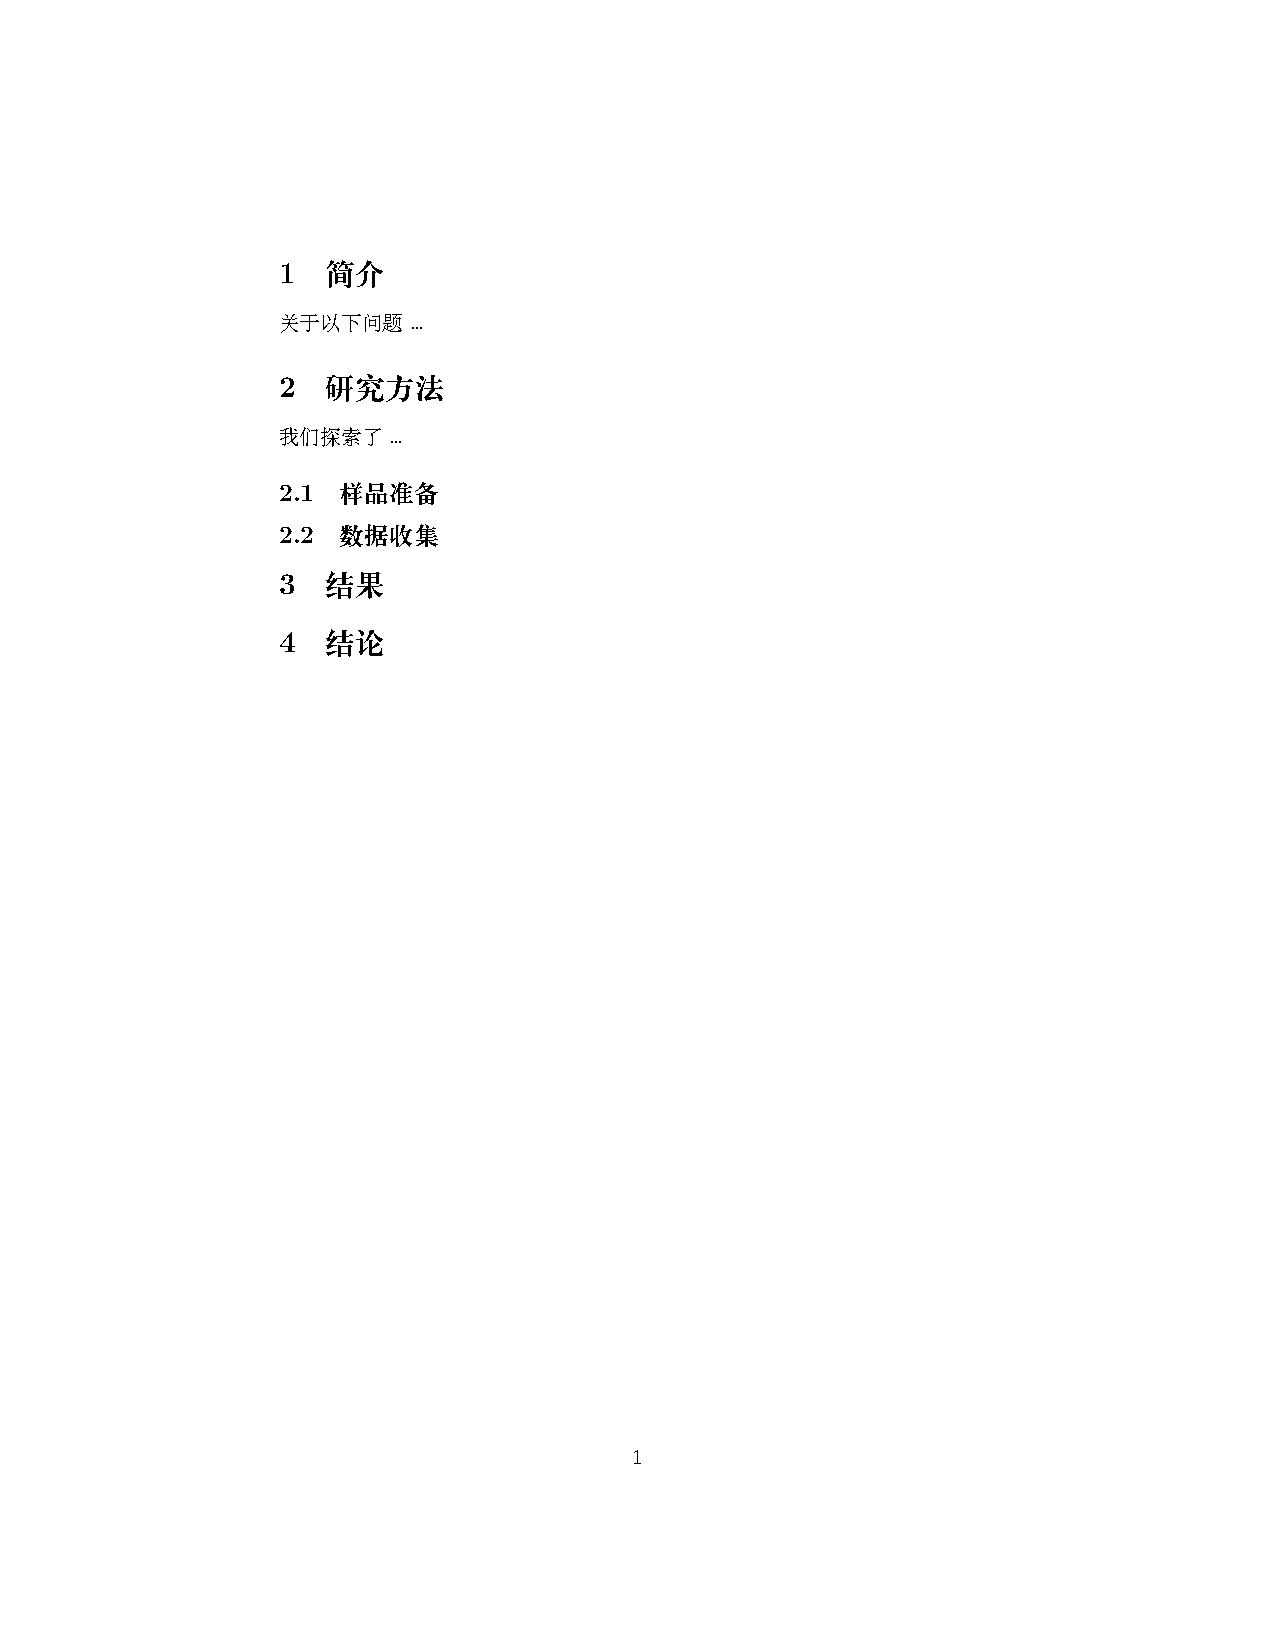
\includegraphics[width=\textwidth,clip,trim=1.5in 6in 4in 1in]{ex-p2-struc-sections.pdf}
\end{minipage}
\end{frame}

%%%%%%%%%%%%%%%%%%%%%%%%%%%%%%%%%%%%%%%%%%%%%%%%%%%%%%%%%%%%%%%%%%%%%%%%%%%%%%%
%%%%%%%%%%%%%%%%%%%%%%%%%%%%%%%%%%%%%%%%%%%%%%%%%%%%%%%%%%%%%%%%%%%%%%%%%%%%%%%
%%%%%%%%%%%%%%%%%%%%%%%%%%%%%%%%%%%%%%%%%%%%%%%%%%%%%%%%%%%%%%%%%%%%%%%%%%%%%%%
\subsection{标签和引用}
\begin{frame}[fragile]{\insertsubsection}
\begin{itemize}{\small
\item 用 \cmdbs{label} 和 \cmdbs{ref} 自动编号
\item \bftt{amsmath} 宏包提供 \cmdbs{eqref} 以引用表达式。
}\end{itemize}
\begin{minipage}{0.55\linewidth}
\inputminted[fontsize=\scriptsize,frame=single,resetmargins]{latex}%
  {ex-p2-struc-crossref.tex}
\end{minipage}
\begin{minipage}{0.35\linewidth}

\includegraphics[width=\textwidth,clip,trim=1.8in 6in 1.6in 1in]{ex-p2-struc-crossref.pdf}
\end{minipage}
\end{frame}

%%%%%%%%%%%%%%%%%%%%%%%%%%%%%%%%%%%%%%%%%%%%%%%%%%%%%%%%%%%%%%%%%%%%%%%%%%%%%%%
%%%%%%%%%%%%%%%%%%%%%%%%%%%%%%%%%%%%%%%%%%%%%%%%%%%%%%%%%%%%%%%%%%%%%%%%%%%%%%%
%%%%%%%%%%%%%%%%%%%%%%%%%%%%%%%%%%%%%%%%%%%%%%%%%%%%%%%%%%%%%%%%%%%%%%%%%%%%%%
\subsection{练习}
\begin{frame}[fragile]{多层文档练习}

\begin{block}{用 \LaTeX 输入这篇短论文:
\footnote{英文版来自 \url{http://pdos.csail.mit.edu/scigen/},一个论文随机生成器,中文版是笠翁对韵,三字经和千字文。}}
\begin{center}
\fbox{\href{\fileuri/exercise-part2-structure-sol.pdf}{%
点击打开文档}}
\end{center}
你的目标就是这样的文档。用 \cmdbs{ref} 和 \cmdbs{eqref};不要在文本中直接写章节和方程编号。
\end{block}
\vskip 2ex
\begin{center}
\fbox{\href{\wlnewdoc{exercise-part2-structure.tex}}{%
点此在 \wllogo{} 中打开该练习的源码}}
\end{center}

\begin{itemize}
\item 试过后,
\fbox{\href{\wlnewdoc{exercise-part2-structure-sol.tex}}{%
这里有我的代码}}.
\end{itemize}
\end{frame}

%%%%%%%%%%%%%%%%%%%%%%%%%%%%%%%%%%%%%%%%%%%%%%%%%%%%%%%%%%%%%%%%%%%%%%%%%%%%%%%
%%%%%%%%%%%%%%%%%%%%%%%%%%%%%%%%%%%%%%%%%%%%%%%%%%%%%%%%%%%%%%%%%%%%%%%%%%%%%%%
%%%%%%%%%%%%%%%%%%%%%%%%%%%%%%%%%%%%%%%%%%%%%%%%%%%%%%%%%%%%%%%%%%%%%%%%%%%%%%%
\section{图表}

%%%%%%%%%%%%%%%%%%%%%%%%%%%%%%%%%%%%%%%%%%%%%%%%%%%%%%%%%%%%%%%%%%%%%%%%%%%%%%%
%%%%%%%%%%%%%%%%%%%%%%%%%%%%%%%%%%%%%%%%%%%%%%%%%%%%%%%%%%%%%%%%%%%%%%%%%%%%%%%
%%%%%%%%%%%%%%%%%%%%%%%%%%%%%%%%%%%%%%%%%%%%%%%%%%%%%%%%%%%%%%%%%%%%%%%%%%%%%%%
\begin{frame}{大纲}
\begin{multicols}{2}
\tableofcontents[currentsection]
\end{multicols}
\end{frame}

%%%%%%%%%%%%%%%%%%%%%%%%%%%%%%%%%%%%%%%%%%%%%%%%%%%%%%%%%%%%%%%%%%%%%%%%%%%%%%%
%%%%%%%%%%%%%%%%%%%%%%%%%%%%%%%%%%%%%%%%%%%%%%%%%%%%%%%%%%%%%%%%%%%%%%%%%%%%%%%
%%%%%%%%%%%%%%%%%%%%%%%%%%%%%%%%%%%%%%%%%%%%%%%%%%%%%%%%%%%%%%%%%%%%%%%%%%%%%%%
\subsection{图象}
\begin{frame}[fragile]{\insertsubsection}
\begin{itemize}
\item 需要 \bftt{graphicx} 宏包提供
\cmdbs{includegraphics} 命令
\item 支持包括 JPEG, PNG 和 (大多数) PDF格式的图像.
\end{itemize}
\begin{exampletwouptiny}

\includegraphics[
  width=0.5\textwidth]{gerbil}


\includegraphics[
  width=0.3\textwidth,
  angle=270]{gerbil}
\end{exampletwouptiny}

\tiny{图象使用许可:\href{https://pixabay.com/en/animal-apple-attractive-beautiful-1239390/}{CC0}}
\end{frame}

%%%%%%%%%%%%%%%%%%%%%%%%%%%%%%%%%%%%%%%%%%%%%%%%%%%%%%%%%%%%%%%%%%%%%%%%%%%%%%%
%%%%%%%%%%%%%%%%%%%%%%%%%%%%%%%%%%%%%%%%%%%%%%%%%%%%%%%%%%%%%%%%%%%%%%%%%%%%%%%
%%%%%%%%%%%%%%%%%%%%%%%%%%%%%%%%%%%%%%%%%%%%%%%%%%%%%%%%%%%%%%%%%%%%%%%%%%%%%%%
\begin{frame}[fragile]{插曲:非必需参数}
\begin{itemize}
\item 非必需参数都放在方括号 \keystrokebftt{[} \keystrokebftt{]} 里,而非花括号 \keystrokebftt{\{} \keystrokebftt{\}}。
\item \cmdbs{includegraphics} 命令有许多参数可调整。这些非必需参数可以调整图像显示的方式。比如\bftt{width=0.3\cmdbs{textwidth}} 使图像宽度变为文段宽(\cmdbs{textwidth})乘以$0.3$。
\item \cmdbs{documentclass} 也有可选参数。比如:
\mint{latex}|\documentclass[12pt,twocolumn]{article}|
\vskip 3ex
将字体放大至12pt(小四)并用\bftt{twocolomn}分成两栏.
\item 去哪里查找这些可调整的参数?片末有资源。
\end{itemize}
\end{frame}

%%%%%%%%%%%%%%%%%%%%%%%%%%%%%%%%%%%%%%%%%%%%%%%%%%%%%%%%%%%%%%%%%%%%%%%%%%%%%%%
%%%%%%%%%%%%%%%%%%%%%%%%%%%%%%%%%%%%%%%%%%%%%%%%%%%%%%%%%%%%%%%%%%%%%%%%%%%%%%%
%%%%%%%%%%%%%%%%%%%%%%%%%%%%%%%%%%%%%%%%%%%%%%%%%%%%%%%%%%%%%%%%%%%%%%%%%%%%%%%
\subsection[fragile]{图片位置/Floats}
\begin{frame}{\insertsubsection}
\begin{itemize}
\item \LaTeX{} 允许自定义图片位置 (“浮动”格式).
\item 你也可以添加图注
\cmdbs{ref}.
\end{itemize}
\begin{minipage}{0.55\linewidth}
\inputminted[fontsize=\scriptsize,frame=single,resetmargins]{latex}%
  {ex-p2-media-graphics.tex}
\end{minipage}
\begin{minipage}{0.35\linewidth}
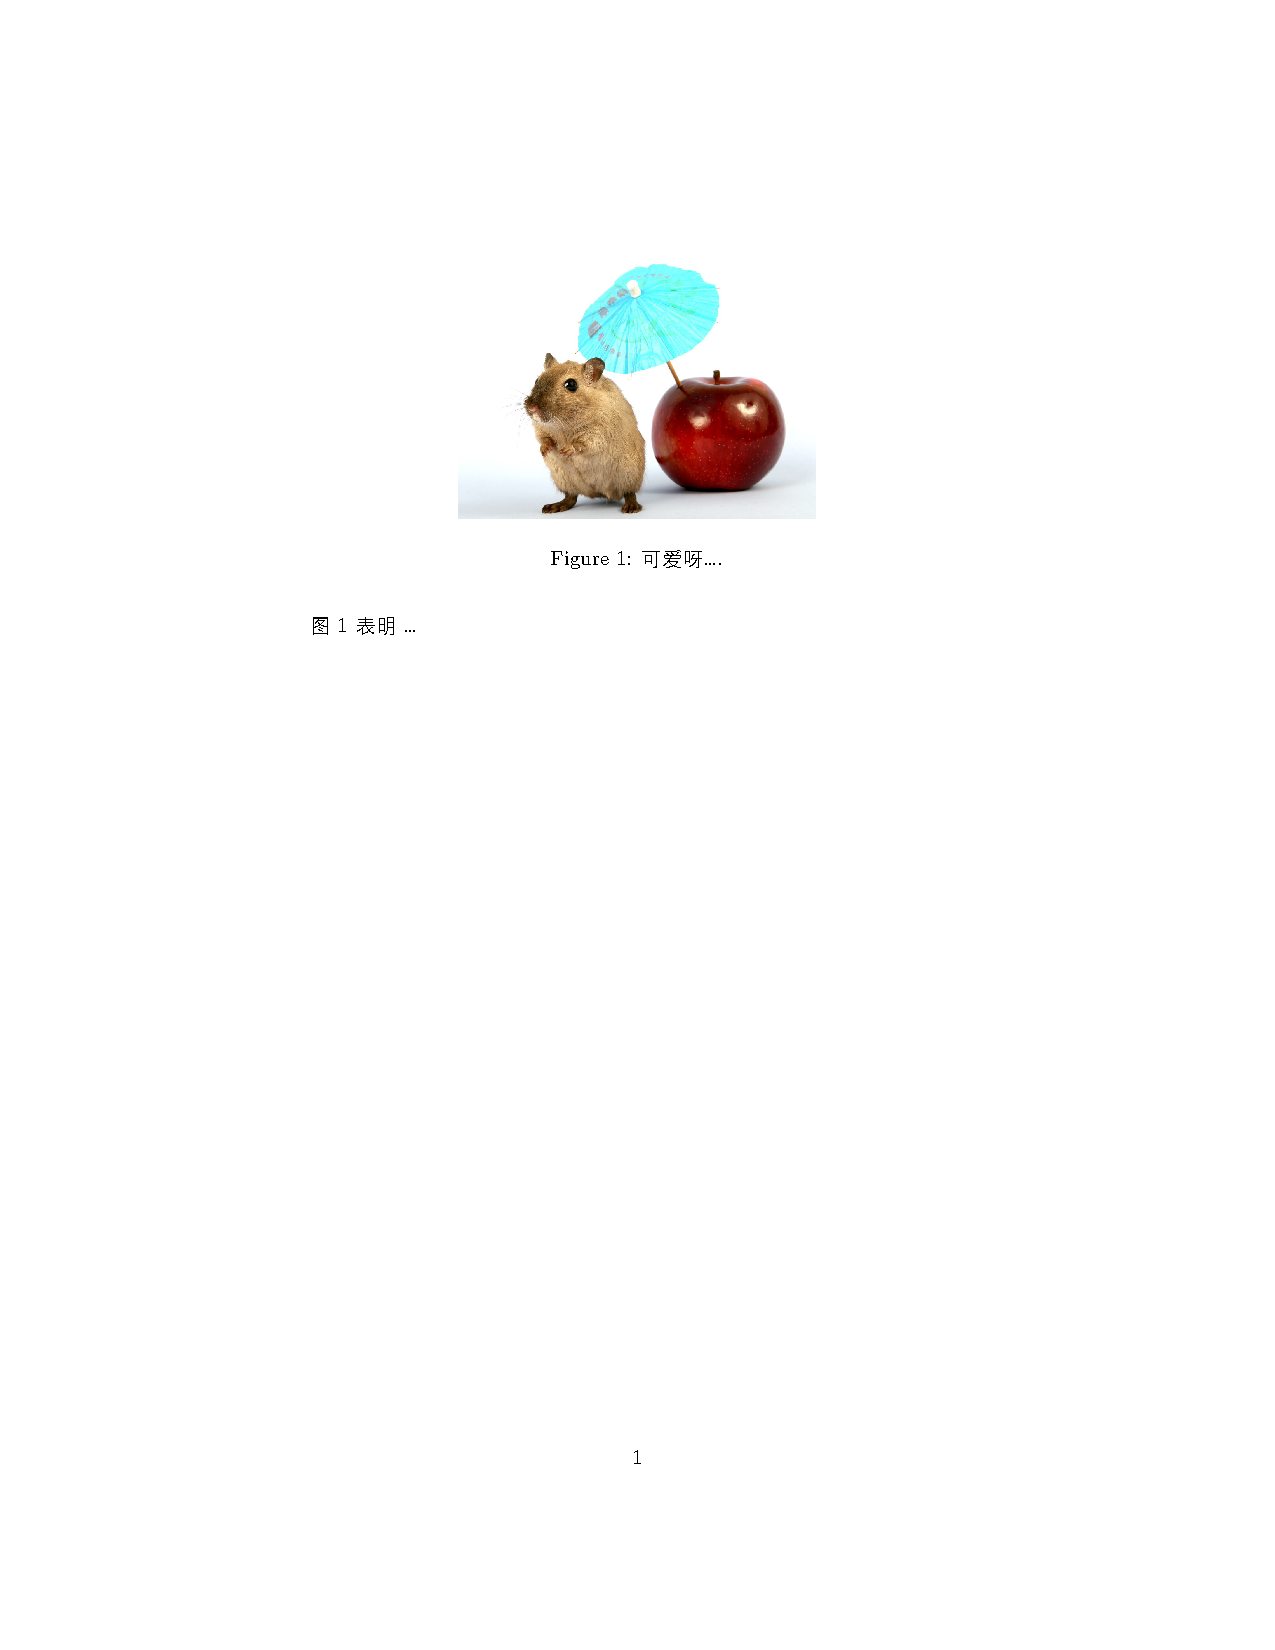
\includegraphics[width=\textwidth,clip,trim=2in 5in 3in 1in]{ex-p2-media-graphics.pdf}
\end{minipage}

\tiny{图象使用许可:\href{https://pixabay.com/en/animal-apple-attractive-beautiful-1239390/}{CC0}}
\end{frame}

%%%%%%%%%%%%%%%%%%%%%%%%%%%%%%%%%%%%%%%%%%%%%%%%%%%%%%%%%%%%%%%%%%%%%%%%%%%%%%%
%%%%%%%%%%%%%%%%%%%%%%%%%%%%%%%%%%%%%%%%%%%%%%%%%%%%%%%%%%%%%%%%%%%%%%%%%%%%%%%
%%%%%%%%%%%%%%%%%%%%%%%%%%%%%%%%%%%%%%%%%%%%%%%%%%%%%%%%%%%%%%%%%%%%%%%%%%%%%%%
\subsection{制表}
\begin{frame}[fragile]{\insertsubsection}
\begin{itemize}
\item \LaTeX{} 制表,习惯了其实很方便。
\item 用 \bftt{tabularx} 宏包的 \bftt{tabular}表格情境。 
\item 花括号里是各栏对齐方式——\textbf{l}eft左对齐, \textbf{r}ight右对齐, \textbf{r}ight右对齐.
\begin{exampletwouptiny}
\begin{tabular}{lrr}
物品   & 数量 & 单价 \$ \\
冬瓜   & 1   & 199.99  \\
南瓜   & 2   & 399.99  \\
西瓜   & 3   & 19.99   \\
\end{tabular}
\end{exampletwouptiny}
\item 这部分也能设置纵向分割线; \cmdbs{hline} 生成横向分割线。
\begin{exampletwouptiny}
\begin{tabular}{|l|r|r|} \hline
物品   & 数量 & 单价 \$ \\\hline
冬瓜   & 1   & 199.99  \\
南瓜   & 2   & 399.99  \\
西瓜   & 3   & 19.99   \\\hline
\end{tabular}
\end{exampletwouptiny}
\item 用and符号 \keystrokebftt{\&} 分栏,双反斜线 \keystrokebftt{\bs}\keystrokebftt{\bs} 换行 (和第一部分 \bftt{align*} 情境中格式一样).
\end{itemize}
\end{frame}

%%%%%%%%%%%%%%%%%%%%%%%%%%%%%%%%%%%%%%%%%%%%%%%%%%%%%%%%%%%%%%%%%%%%%%%%%%%%%%%
%%%%%%%%%%%%%%%%%%%%%%%%%%%%%%%%%%%%%%%%%%%%%%%%%%%%%%%%%%%%%%%%%%%%%%%%%%%%%%%
%%%%%%%%%%%%%%%%%%%%%%%%%%%%%%%%%%%%%%%%%%%%%%%%%%%%%%%%%%%%%%%%%%%%%%%%%%%%%%%
\addtocontents{toc}{\newpage}
\section{引用}

%%%%%%%%%%%%%%%%%%%%%%%%%%%%%%%%%%%%%%%%%%%%%%%%%%%%%%%%%%%%%%%%%%%%%%%%%%%%%%%
%%%%%%%%%%%%%%%%%%%%%%%%%%%%%%%%%%%%%%%%%%%%%%%%%%%%%%%%%%%%%%%%%%%%%%%%%%%%%%%
%%%%%%%%%%%%%%%%%%%%%%%%%%%%%%%%%%%%%%%%%%%%%%%%%%%%%%%%%%%%%%%%%%%%%%%%%%%%%%%
\begin{frame}{大纲}
\begin{multicols}{2}
\tableofcontents[currentsection]
\end{multicols}
\end{frame}

%%%%%%%%%%%%%%%%%%%%%%%%%%%%%%%%%%%%%%%%%%%%%%%%%%%%%%%%%%%%%%%%%%%%%%%%%%%%%%%
%%%%%%%%%%%%%%%%%%%%%%%%%%%%%%%%%%%%%%%%%%%%%%%%%%%%%%%%%%%%%%%%%%%%%%%%%%%%%%%
%%%%%%%%%%%%%%%%%%%%%%%%%%%%%%%%%%%%%%%%%%%%%%%%%%%%%%%%%%%%%%%%%%%%%%%%%%%%%%%
\subsection{bib\TeX}
\begin{frame}[fragile]{\insertsubsection{} 1}
\begin{itemize}
\item 要想用\LaTeX{}自动处理脚注,文献页等,需先把参考文献用“bibtex”数据库格式放在一个 \bftt{.bib} 文档里:
\inputminted[fontsize=\scriptsize,frame=single]{latex}{ex-p2-bib.bib}
\item 大多数引用处理器都能生成bibtex格式文件。
\end{itemize}
\end{frame}

%%%%%%%%%%%%%%%%%%%%%%%%%%%%%%%%%%%%%%%%%%%%%%%%%%%%%%%%%%%%%%%%%%%%%%%%%%%%%%%
%%%%%%%%%%%%%%%%%%%%%%%%%%%%%%%%%%%%%%%%%%%%%%%%%%%%%%%%%%%%%%%%%%%%%%%%%%%%%%%
%%%%%%%%%%%%%%%%%%%%%%%%%%%%%%%%%%%%%%%%%%%%%%%%%%%%%%%%%%%%%%%%%%%%%%%%%%%%%%%
\begin{frame}[fragile]{\insertsubsection{} 2}
\begin{itemize}
\item \bftt{.bib} 文档中的每一项都有一个关键字 \emph{key} 可供在文内引用。如 \bftt{Jacobson1999Towards} 就是这篇论文的关键字:
\begin{minted}[fontsize=\small,frame=single]{latex}
@Article{Jacobson1999Towards,
  author = {Van Jacobson},
  ...
}
\end{minted}
\item 最好用作者/年份/标题作为关键字。
\item \LaTeX{} 可以自动将文内引用的资料按统一格式处理,并在文尾生成单独页面;它预存了常用的格式,也支持自定义。
\end{itemize}
\end{frame}

%%%%%%%%%%%%%%%%%%%%%%%%%%%%%%%%%%%%%%%%%%%%%%%%%%%%%%%%%%%%%%%%%%%%%%%%%%%%%%%
%%%%%%%%%%%%%%%%%%%%%%%%%%%%%%%%%%%%%%%%%%%%%%%%%%%%%%%%%%%%%%%%%%%%%%%%%%%%%%%
%%%%%%%%%%%%%%%%%%%%%%%%%%%%%%%%%%%%%%%%%%%%%%%%%%%%%%%%%%%%%%%%%%%%%%%%%%%%%%%
\begin{frame}[fragile]{\insertsubsection{} 3}
\begin{itemize}
\item 用 \bftt{natbib} 宏包\footnote{T还有一个功能更多的 \bftt{biblatex} 宏包。不过大多数文档还是用
  \bftt{natbib}。} 处理 \cmdbs{citet} 和 \cmdbs{citep}。
\item 在文尾插入 \cmdbs{bibliography} 命令并设置引用格式 \cmdbs{bibliographystyle}。
\end{itemize}
\begin{minipage}{0.55\linewidth}
\inputminted[fontsize=\scriptsize,frame=single,resetmargins]{latex}%
  {ex-p2-bib.tex}
\end{minipage}
\begin{minipage}{0.35\linewidth}
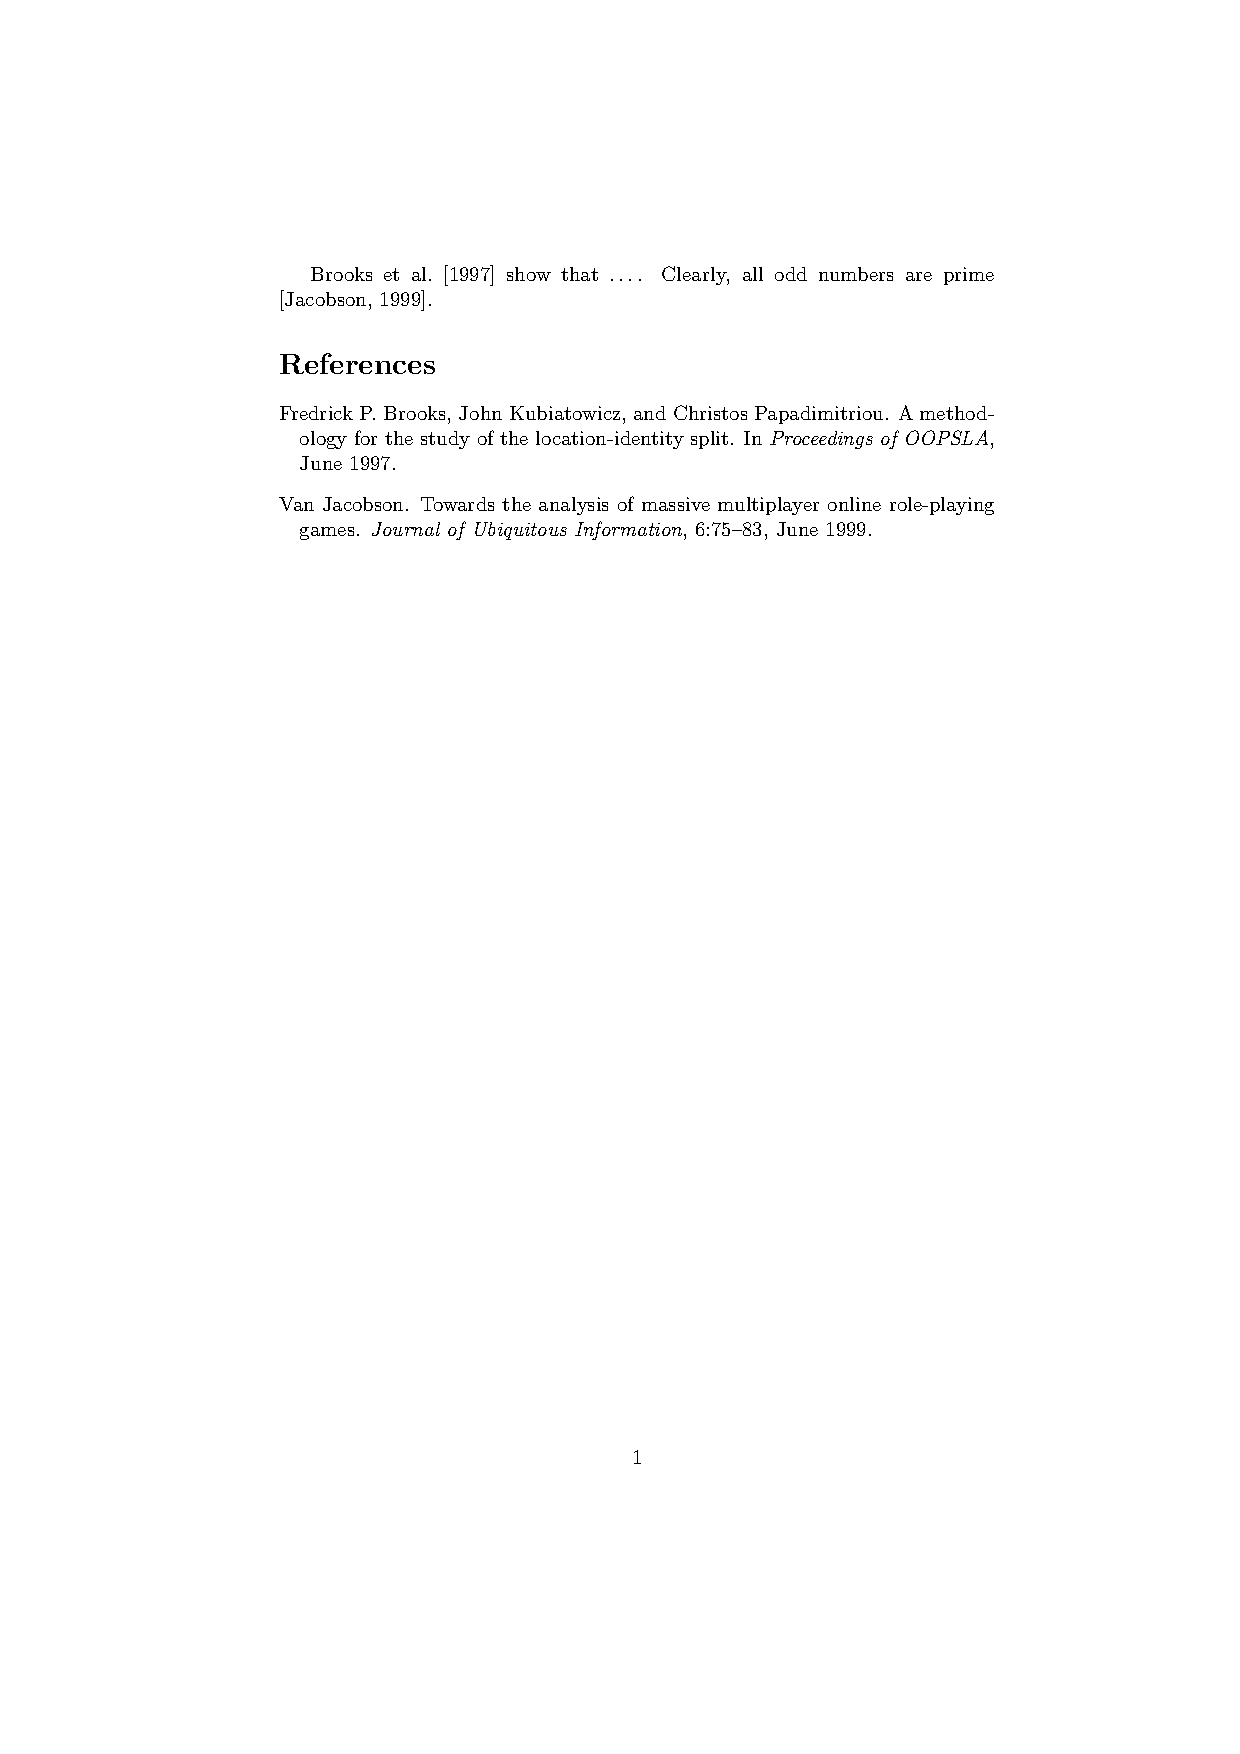
\includegraphics[width=\textwidth,clip,trim=1.8in 5in 1.8in 1in]{ex-p2-bib.pdf}
\end{minipage}
\end{frame}

%%%%%%%%%%%%%%%%%%%%%%%%%%%%%%%%%%%%%%%%%%%%%%%%%%%%%%%%%%%%%%%%%%%%%%%%%%%%%%%
%%%%%%%%%%%%%%%%%%%%%%%%%%%%%%%%%%%%%%%%%%%%%%%%%%%%%%%%%%%%%%%%%%%%%%%%%%%%%%%
%%%%%%%%%%%%%%%%%%%%%%%%%%%%%%%%%%%%%%%%%%%%%%%%%%%%%%%%%%%%%%%%%%%%%%%%%%%%%%%
\subsection{练习}
\begin{frame}[fragile]{练习:组装文档}

为之前练习中的论文添加图片和引用部分。

\begin{enumerate}
\item 下载示例文档到本地

\begin{center}
\fbox{\href{\fileuri/gerbil.jpg?dl=1}{点此下载例图}}

\fbox{\href{\fileuri/exercise-part2-bib?dl=1}{点此下载bib文档示例}}
\end{center}

\item 上传到Overleaf (打开Project菜单).

\end{enumerate}
\end{frame}

%%%%%%%%%%%%%%%%%%%%%%%%%%%%%%%%%%%%%%%%%%%%%%%%%%%%%%%%%%%%%%%%%%%%%%%%%%%%%%%
%%%%%%%%%%%%%%%%%%%%%%%%%%%%%%%%%%%%%%%%%%%%%%%%%%%%%%%%%%%%%%%%%%%%%%%%%%%%%%%
%%%%%%%%%%%%%%%%%%%%%%%%%%%%%%%%%%%%%%%%%%%%%%%%%%%%%%%%%%%%%%%%%%%%%%%%%%%%%%%
\section{就结束啦?}

%%%%%%%%%%%%%%%%%%%%%%%%%%%%%%%%%%%%%%%%%%%%%%%%%%%%%%%%%%%%%%%%%%%%%%%%%%%%%%%
%%%%%%%%%%%%%%%%%%%%%%%%%%%%%%%%%%%%%%%%%%%%%%%%%%%%%%%%%%%%%%%%%%%%%%%%%%%%%%%
%%%%%%%%%%%%%%%%%%%%%%%%%%%%%%%%%%%%%%%%%%%%%%%%%%%%%%%%%%%%%%%%%%%%%%%%%%%%%%%
\begin{frame}{大纲}
\begin{multicols}{2}
\tableofcontents[currentsection]
\end{multicols}
\end{frame}

%%%%%%%%%%%%%%%%%%%%%%%%%%%%%%%%%%%%%%%%%%%%%%%%%%%%%%%%%%%%%%%%%%%%%%%%%%%%%%%
%%%%%%%%%%%%%%%%%%%%%%%%%%%%%%%%%%%%%%%%%%%%%%%%%%%%%%%%%%%%%%%%%%%%%%%%%%%%%%%
%%%%%%%%%%%%%%%%%%%%%%%%%%%%%%%%%%%%%%%%%%%%%%%%%%%%%%%%%%%%%%%%%%%%%%%%%%%%%%%
\subsection{更多技巧}
\begin{frame}[fragile]{\insertsubsection}
\begin{itemize}
\item 添加 \cmdbs{tableofcontents} 命令,可自动提取 \cmdbs{section} 中的信息并生成目录.

\item 把文档类型 \cmdbs{documentclass} 改为
\mint{latex}!\documentclass{scrartcl}!
或\mint{latex}!\documentclass[12pt]{IEEEtran}!

\item 为复杂的方程自定义命令:
\begin{exampletwouptiny}
\newcommand{\rperf}{%
  \rho_{\text{perf}}}
$$
\rperf = {\bf c}'{\bf X} + \varepsilon
$$
\end{exampletwouptiny}
\end{itemize}
\end{frame}

%%%%%%%%%%%%%%%%%%%%%%%%%%%%%%%%%%%%%%%%%%%%%%%%%%%%%%%%%%%%%%%%%%%%%%%%%%%%%%%
%%%%%%%%%%%%%%%%%%%%%%%%%%%%%%%%%%%%%%%%%%%%%%%%%%%%%%%%%%%%%%%%%%%%%%%%%%%%%%%
%%%%%%%%%%%%%%%%%%%%%%%%%%%%%%%%%%%%%%%%%%%%%%%%%%%%%%%%%%%%%%%%%%%%%%%%%%%%%%%
\subsection{常用宏包}
\begin{frame}{\insertsubsection}
\begin{itemize}
\item \bftt{beamer}: 做幻灯片(就是我)
\item \bftt{todonotes}: 注释和备忘
\item \bftt{tikz}: 制图惊艳
\item \bftt{pgfplots}: \LaTeX 绘图
\item \bftt{listings}: 在 \LaTeX 中显示源码
\item \bftt{spreadtab}: 在 \LaTeX 中制表
\item \bftt{gchords}, \bftt{guitar}: 吉他和弦和图氏记谱
\item \bftt{cwpuzzle}: 填字游戏
\end{itemize}
\url{https://www.overleaf.com/latex/examples} 和 \url{http://texample.net}
上有以上(大多数)宏包的示例。
\end{frame}

%%%%%%%%%%%%%%%%%%%%%%%%%%%%%%%%%%%%%%%%%%%%%%%%%%%%%%%%%%%%%%%%%%%%%%%%%%%%%%%
%%%%%%%%%%%%%%%%%%%%%%%%%%%%%%%%%%%%%%%%%%%%%%%%%%%%%%%%%%%%%%%%%%%%%%%%%%%%%%%
%%%%%%%%%%%%%%%%%%%%%%%%%%%%%%%%%%%%%%%%%%%%%%%%%%%%%%%%%%%%%%%%%%%%%%%%%%%%%%%
\subsection{安装\LaTeX{}}
\begin{frame}{\insertsubsection}
\begin{itemize}
\item 若想在自己电脑上编译 \LaTeX{},需使用 \LaTeX{}
\emph{distribution}(发布版)。发布版包括一个 \bftt{latex} 编译器及(通常)上千个宏包.
\begin{itemize}
\item Windows操作系统: \href{http://miktex.org/}{Mik\TeX} or \href{http://tug.org/texlive/}{\TeX Live}
\item Linux: \href{http://tug.org/texlive/}{\TeX Live}
\item Mac: \href{http://tug.org/mactex/}{Mac\TeX}
\end{itemize}
\item 需要一个支持\LaTeX{} 的文本编辑器。\url{http://en.wikipedia.org/wiki/Comparison_of_TeX_editors} 上有不少选择。
\item 需要进一步学习 \bftt{latex} 和有关工具——下一页提供了一些资料。
\end{itemize}
\end{frame}

%%%%%%%%%%%%%%%%%%%%%%%%%%%%%%%%%%%%%%%%%%%%%%%%%%%%%%%%%%%%%%%%%%%%%%%%%%%%%%%
%%%%%%%%%%%%%%%%%%%%%%%%%%%%%%%%%%%%%%%%%%%%%%%%%%%%%%%%%%%%%%%%%%%%%%%%%%%%%%%
%%%%%%%%%%%%%%%%%%%%%%%%%%%%%%%%%%%%%%%%%%%%%%%%%%%%%%%%%%%%%%%%%%%%%%%%%%%%%%%
\subsection{在线资料}
\begin{frame}{\insertsubsection}
\begin{itemize}
\item \href{http://en.wikibooks.org/wiki/LaTeX}{The \LaTeX{} Wikibook} ——实用的教程和参考资料。
\item \href{http://tex.stackexchange.com/}{\TeX{} Stack Exchange} ——先搜索已解决问题再提问;很快就有优质解答。
\item \href{http://www.latex-community.org/}{\LaTeX{} Community} ——庞大用户论坛
\item \href{http://ctan.org/}{Comprehensive \TeX{} Archive Network (CTAN)} ---
包括超四千份宏包和代码说明。
\item 搜索引擎返回的大多都是以上网站。
\end{itemize}
\end{frame}

%%%%%%%%%%%%%%%%%%%%%%%%%%%%%%%%%%%%%%%%%%%%%%%%%%%%%%%%%%%%%%%%%%%%%%%%%%%%%%%
%%%%%%%%%%%%%%%%%%%%%%%%%%%%%%%%%%%%%%%%%%%%%%%%%%%%%%%%%%%%%%%%%%%%%%%%%%%%%%%
%%%%%%%%%%%%%%%%%%%%%%%%%%%%%%%%%%%%%%%%%%%%%%%%%%%%%%%%%%%%%%%%%%%%%%%%%%%%%%%
\begin{frame}
\begin{center}
谢谢观看,祝你 \TeX{}ing 愉快!
\end{center}
\end{frame}

\end{document}

% -- latex understands words, sentences and paragraphs

Words are separated by one or more spaces.  Paragraphs are separated by
one or more blank lines.  The output is not affected by adding extra
spaces or extra blank lines to the input file.

Double quotes are typed like this: ``quoted text''.
Single quotes are typed like this: `single-quoted text'.

Emphasized text is typed like this: \emph{this is emphasized}.
Bold       text is typed like this: \textbf{this is bold}.

-- Adding structure to your document

\section{Hello}

\subsection{World}

\subsection{Foo}

\subsubsection*{Stuff} % star form

\subsubsection*{Results}

-- Labels and cross-references

\label{sec:intro}
\label{sec:method}
\ref{sec:method}

--> maybe introduce the prettyref package here.

-- Mathematics

Inline mathematics: $x + y < 7$.

'Displayed' mathematics:
\begin{equation}
\end{equation}

\begin{equation*}
\end{equation*}

\begin{align}
\end{align}

-- Figures

- Need the graphicx package.

- here we can start introducing options

\includegraphics[width=\textwidth]{}

- where do you find out about these options? --> link to the Wikibook

-- Floating Figures

\begin{figure}
\includegraphics{...}
\caption{\label{}Here is a caption.}
\end{figure}

-- Tables

- not the nicest part of LaTeX

\usepackage{tabularx}

\begin{tabular}{llr}
Item & Quantity & Price (\$) & Amount
Widget & 1 &
\end{tabular}

Bonus points: check out the fp package and the spreadtab package.

-- Document Classes

a .cls file

article

some journal templates come with one

-- Bibliographies



-- For Typesetting Geeks

- dashes: -, --, ---

- ellipsis.

- controlling spaces: ~, \ , \,, \@

- spacing after periods (et al., etc.)

- Nested quotation marks: ``\,`
\vskip 2ex
\item Use the \emph{star form} to display an equation without a number.
\begin{exampletwouptiny}
\begin{equation*}
F(x) = \int_{a}^{x}{f(t) dt}
\end{equation*}
\end{exampletwouptiny}

\begin{itemize}
\item \bftt{equation} and \bftt{equation*} are called \emph{environments}.
\begin{itemize}
  \item The \cmdbs{begin} and \cmdbs{end} commands define the environment.
  \item The \cmd{\$} also starts and ends an environment.
  \item Some commands are defined only within certain environments.
  \item Some commands behave differently in different environments.
\end{itemize}
\end{itemize}
\end{block}
\begin{center}
\fbox{\href{http://ctan.org/}{The Comprehensive \TeX Archive Network (CTAN)}}
\end{center}

%%%%%%%%%%%%%%%%%%%%%%%%%%%%%%%%%%%%%%%%%%%%%%%%%%%%%%%%%%%%%%%%%%%%%%%%%%%%%%%
%%%%%%%%%%%%%%%%%%%%%%%%%%%%%%%%%%%%%%%%%%%%%%%%%%%%%%%%%%%%%%%%%%%%%%%%%%%%%%%
%%%%%%%%%%%%%%%%%%%%%%%%%%%%%%%%%%%%%%%%%%%%%%%%%%%%%%%%%%%%%%%%%%%%%%%%%%%%%%%
\subsection{Typography tweaks}
\begin{frame}{\insertsubsection}
\begin{tabular}{lll}
& character name & used mainly for \ldots \\\hline
\bftt{\bs} & backslash                 & commands, tables \\
\bftt{\{}  & open brace                & commands \\
\bftt{\}}  & close brace               & commands \\
\bftt{\%}  & percent sign              & comments \\
\bftt{\#}  & hash (pound / sharp) sign & custom commands \\
\bftt{\$}  & dollar sign               & equations \\
\bftt{\_}  & underscore                & equations (subscripts) \\
\bftt{\^}  & caret                     & equations (superscripts) \\
\bftt{\&}  & ampersand                 & tables \\
\bftt{\~}  & tilde                     & spacing \\
\end{tabular}
\end{frame}

%\item We've used several environments:
%\vskip 1ex
%{\scriptsize
%\begin{tabular}{ll}
%\cmdbs{begin}\bftt{\{document\}}\ldots\cmdbs{end}\bftt{\{document\}} &
%  document environment \\
%\cmdbs{begin}\bftt{\{itemize\}}\ldots\cmdbs{end}\bftt{\{itemize\}} &
%  itemized list environment \\
%\bftt{\$\ldots\$}     & \emph{in-text} math environment \\
%\bftt{\$\$\ldots\$\$} & \emph{displayed} math environment \\
%\cmdbs{begin}\bftt{\{equation\}}\ldots\cmdbs{end}\bftt{\{equation\}} &
%  displayed math environment w/ number
%\end{tabular}
%}
